\documentclass{article}
% \usepackage[spanish]{babel}
% \usepackage{lipsum}
% \usepackage{natbib}
% \usepackage{graphicx}
\usepackage{analysis_orax}
\usepackage{wrapfig}

%------------------Document----------------------------

\begin{document}

%-------------------------TitlePage------------------------
%\begin{titlepage}
%\end{titlepage}

%-------------------------Content------------------------
\section{Body of interest}

\subsubsection{Shape}

     The body considered for the flow analysis using MATLAB is shape of a "Batman Blade".

    \begin{figure}[htb]
    \centering
      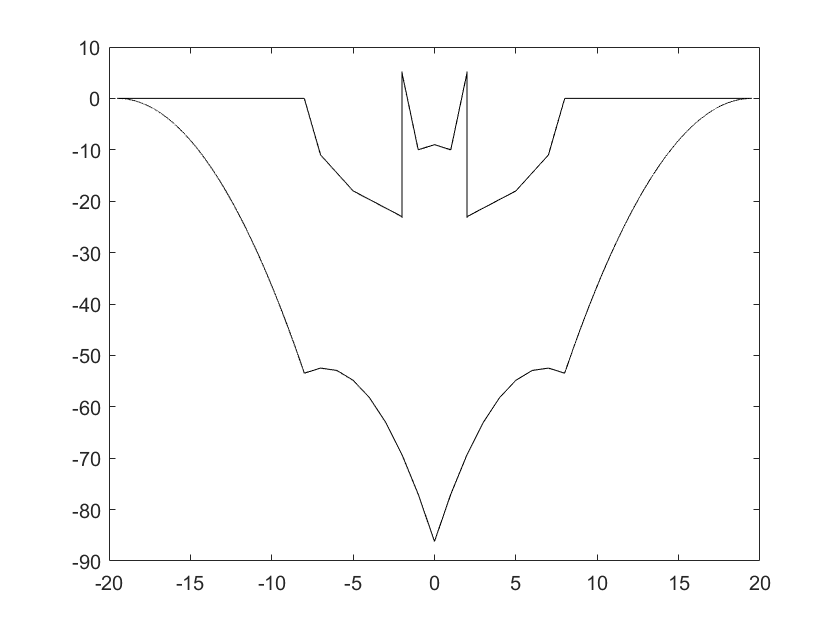
\includegraphics[width=0.7\textwidth]{assets/bat.png}
       \centering
       \vspace{-2mm}
      \textcolor{Orange}{\textbf{\caption{Batman Blade}}}\label{fig:1}
    \end{figure}
    
     \vspace{-3mm}
\subsubsection{Plot}
   We have plotted this body in MATLAB with help of piecewise function, dividing the body in two sections the upper part which consists of straight lines and lower part is a combination of parabolic and elliptic equations.
   
   \begin{wrapfigure}{r}{0.4\textwidth}
   \begin{center}
      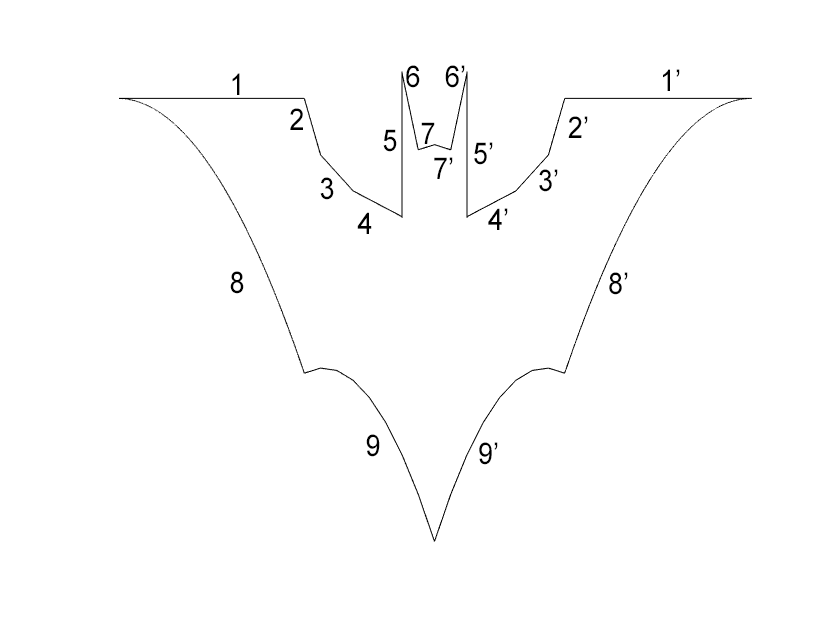
\includegraphics[width=0.5\textwidth]{assets/bat_lines.png}
   \end{center}
   \end{wrapfigure}
   
\vspace{5mm}   
\hspace{20mm} EQUATIONS :  \\ \\
   \vspace{1mm}
$(1)  \hspace{5mm}   x \epsilon\ [-19.48,-8]\hspace{8mm} y(x)= 0 \\ \vspace{1mm}
(2)\hspace{5mm} x \epsilon\ [-8,-7]\hspace{15mm} y(x)= 11x-88  \\ \vspace{1mm}
(3)\hspace{5mm} x \epsilon\ [-7,-5]\hspace{15mm} y(x)= -3.7(x+7)-11  \\ \vspace{1mm}
(4)\hspace{5mm} x \epsilon\ [-5,-2.1]\hspace{12mm} y(x)= -1.67(x+5)-18  \\ \vspace{1mm}
(5)\hspace{5mm} x \epsilon\ [-2.1,-2]\hspace{12mm} y(x)= -15(x+1)-10  \\ \vspace{1mm}
(6)\hspace{5mm} x \epsilon\ [-2,-1]\hspace{15mm} y(x)= -(|x|-1)-10  \\ \vspace{1mm}
(7)\hspace{5mm} x \epsilon\ [-1,0]\hspace{18mm} y(x)= 15(x-1)-10  \\ \vspace{1mm}
(8)\hspace{5mm} x \epsilon\ [-19.48,-8]\hspace{9mm} y(x)= -0.5*(0.9x+17.54)^2  \\ \vspace{1mm}
(9) \hspace{5mm} x \epsilon\ [-8,0]\hspace{18mm} y(x)= 3\sqrt{(64-x^2)} \vspace{3mm} \\   
$
 Rest 9 Equations are just reflection of these in Y-aixs because our body is symmetric about Y-axis.
%-------------------------Content------------------------
\section{Computation}

\subsubsection{Panels and Control Points}
    Flow analysis can be done with different number of panels in our model.
    Although number of panels for upper part are fixed (14) as each straight line is considered as a panel, still total number of panels can be changed by changing number of panels in lower part.
    
    \vspace{8mm}
    \hspace{20mm}
    Here are some examples showing number of panels and control points.
    \vspace{-1mm}

    \begin{figure}[htb]
    \centering  
      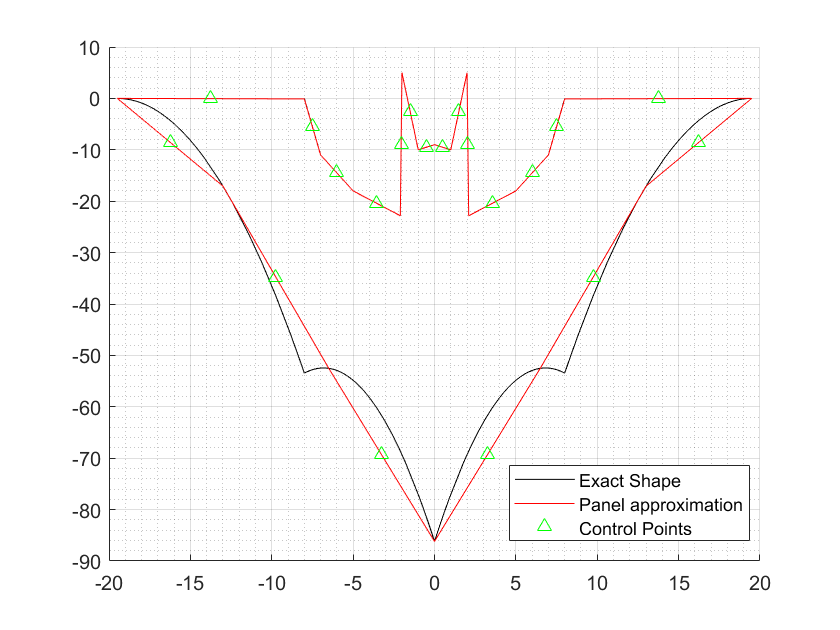
\includegraphics[width=0.45\textwidth]{assets/n20.png}
      %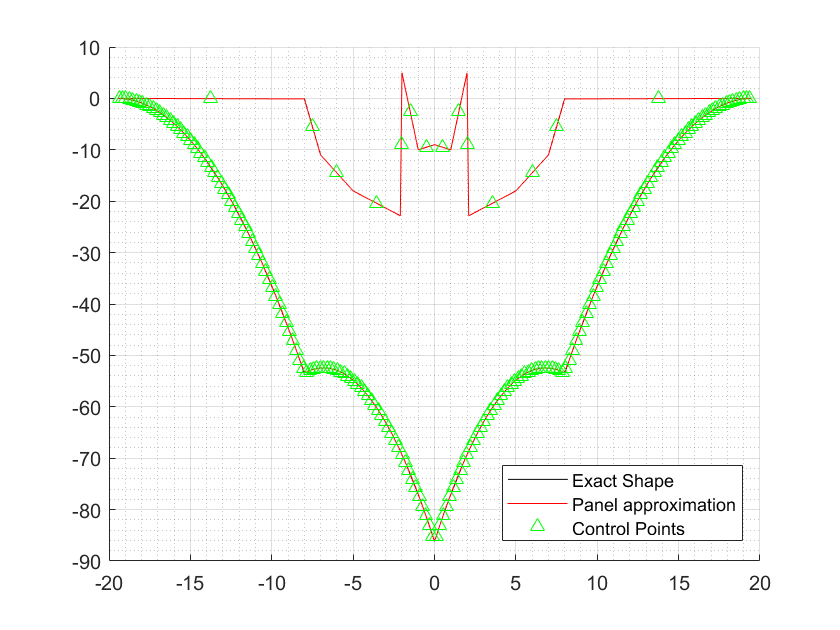
\includegraphics[width=0.3\textwidth]{assets/n200.png}
      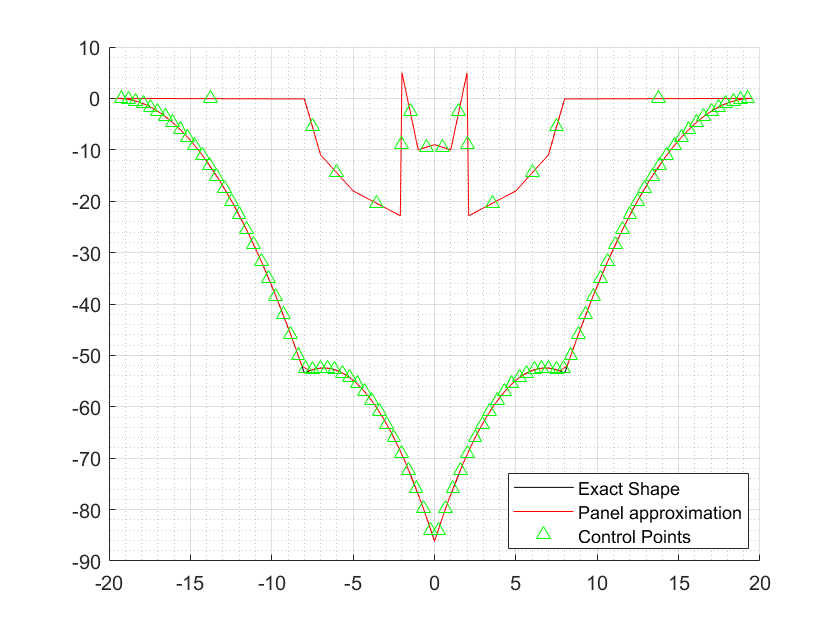
\includegraphics[width=0.45\textwidth]{assets/n100.png}
       \centering
       \\  \vspace{2mm}
             \textcolor{Orange}{n=20}
               \hspace{60mm} 
                 \textcolor{Orange}{n=100}
                 \\
                  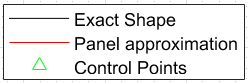
\includegraphics[width=0.3\textwidth]{assets/legends.png}
       \vspace{-2mm}
    \end{figure}
    
\subsubsection{Velocity Vector on Body Surface}
\vspace{-5mm}
    \begin{figure}[htb]
    \centering  
      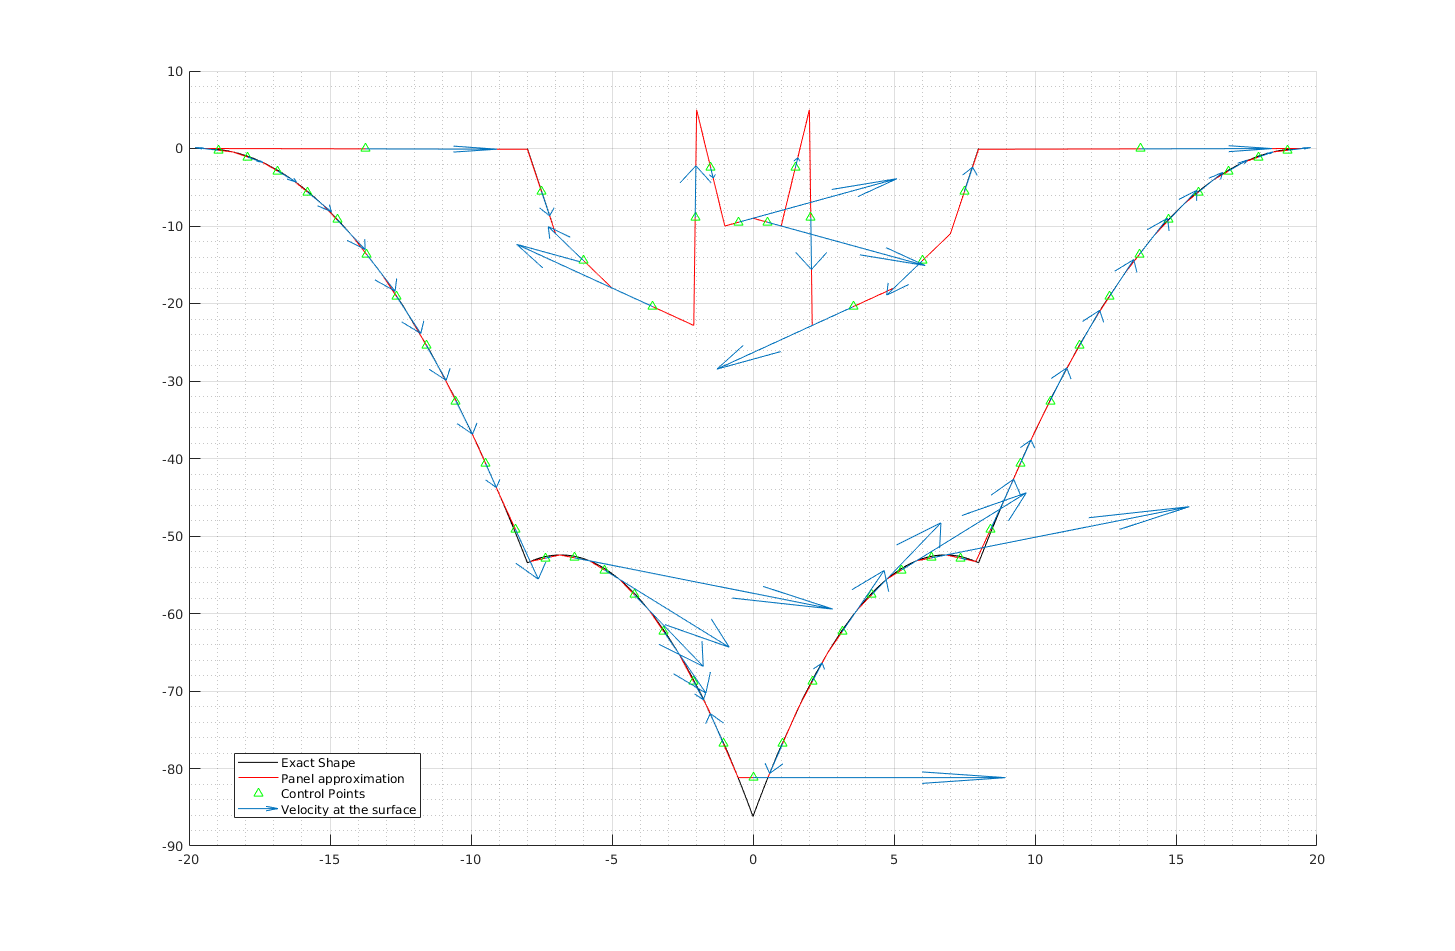
\includegraphics[width=0.8    \textwidth]{assets/velocity_field.png}
       \centering
    \end{figure}
  
%-------------------------Content------------------------
\section{Verification and Debugging}

\subsubsection{Code Verification}

Code is verified by running the code for cylinder and comparing the results with that of \\  \textbf{Example 3.19 J.D Andreson}
\end{document}


